\documentclass[12pt, a4paper]{report}
\usepackage{fontspec}

% Fonts
\defaultfontfeatures{Mapping=tex-text}
\setromanfont [Ligatures={Common},Numbers={OldStyle}]{Adobe Caslon Pro}
\setmonofont[Scale=0.8]{Monaco} 
\setsansfont[Scale=0.9]{Optima Regular}

\usepackage[latin1]{inputenc}

% Headings
\usepackage{sectsty} 
\usepackage[normalem]{ulem} 
\sectionfont{\rmfamily\mdseries\Large} 
\subsectionfont{\rmfamily\mdseries\scshape\normalsize} 
\subsubsectionfont{\rmfamily\bfseries\upshape\normalsize} 

% PDF Setup
\usepackage[dvipdfm, bookmarks, colorlinks, breaklinks, pdftitle={Projectverslag},pdfauthor={Mark Mulder}]{hyperref}  
\hypersetup{linkcolor=black,citecolor=blue,filecolor=black,urlcolor=black}

% Number pages on the bottom
\pagestyle{plain}

% Use Dutch language so we get correct hyphenation
\usepackage[dutch]{babel}
\selectlanguage{dutch}

\begin{document}

  \thispagestyle{empty}

\begin{flushleft}

  \Huge
  Adviezen ter realisatie van een professionele technische infrastructuur voor webdevelopmentbureaus\\

  \vfill{}
  
  \small
  Mark M. Mulder (2009) \\
  Afstudeerproject Interactieve Media aan de Hogeschool van Amsterdam
  \\\emph{Rights reserved}.  \href{http://creativecommons.org/licenses/by-nc-nd/3.0/nl/}{\textsc{cc-by-nc-nd}}
  
\end{flushleft}

\normalsize

  \tableofcontents

  \chapter{Inleiding}

Voor de afstudeerfase van de opleiding Interactieve Media aan de Hogeschool van Amsterdam is mijn keuze gevallen op het uitvoeren van een project bij het bedrijf waar ik stage had gelopen, namelijk Fullmoon Interactive Solutions te Amsterdam.

Tijdens mijn half jaar durende stageperiode merkte ik af en toe dat men bij Fullmoon regelmatig tegen wat problemen aanliep, wat vooral veroorzaakt wordt door het feit dat er vrij kort op elkaar meerdere mensen waren aangenomen. Met acht vaste werknemers en twee stagiaires verliep het samenwerken daarom niet altijd even goed. Eén van de oorzaken was dat een goed overzicht van de verdeling van de werkzaamheden over de verschillende werknemers ontbrak. Bovendien kwam het regelmatig voor dat, wanneer men aan hetzelfde project bezig was, men per ongeluk werk van anderen overschreef, zodat er veel tijd en inspanning verloren ging.

Omdat ik uit eigen interesse al ervaring had opgedaan met Source Control Management  ({\sc scm}) systemen en veel aandacht besteedde aan mijn eigen workflow, heb ik Fullmoon aangeboden te helpen om hun situatie te kunnen verbeteren.

In mijn rapport getiteld ``Adviezen ter realisatie van een professionele technische infrastructuur voor webdevelopmentbureaus'' zijn de adviezen opgenomen, die zijn opgesteld aan de hand van mijn verrichtingen bij Fullmoon. Uitgangspunt bij dit rapport was om de veranderingen en verbeteringen die inmiddels zijn doorgevoerd bij Fullmoon duidelijk zichtbaar te maken, voor zowel studenten als voor bedrijven die met dezelfde problematiek te maken hebben.

In dit document wordt aan de hand van het adviesrapport in kaart gebracht wat er bij Fullmoon uiteindelijk geïmplementeerd is. Tot slot is er nog een persoonlijk projectverslag, waarin na te lezen is wat ik daadwerkelijk gedaan heb voor dit project.

  \chapter{Implementatie}

In het adviesrapport zijn een vijftal adviezen opgesteld, die ik puntsgewijs behandel, zodat een goed beeld wordt verkregen van wat er gebeurd is bij Fullmoon.

\section{SCM Systeem}

\subsection{Keuze}

Bij het selecteren van het voor Fullmoon meest geschikte {\sc scm} systeem, hebben we rekening gehouden met meerdere eisen. Zo was één van de uitgangspunten dat de nieuwe situatie eenvoudig werkbaar moest zijn voor zowel alle in dienst zijnde medewerkers, als voor nieuwe medewerkers. Het moest dus een niet té ingrijpende verandering veroorzaken.

Omdat het een diverse groep is van designers, programmeurs en projectmanagers, waarbij niet iedereen zich even op het gemak voelt met de commandline, is bij Fullmoon gekozen voor Subversion. Het grote aanbod aan (grafische) tools gaf hierbij de doorslag.

\subsection{Uitwerking}

Bij Fullmoon zijn presentaties en uitleg gegeven over het werken met Subversion door gebruik te maken van het programma SmartSVN. Maar de medewerkers zijn in principe vrij in de keuze voor een programma om met Subversion te werken.

Er is een server in gebruik genomen om de Subversion repository te huisvesten. Op dezelfde server draait ook een webserver waarop alle projecten terug te zien zijn. Zo is er een centrale plek waar iedereen de laatste versie van het project kan bekijken om deze eventueel te testen. Ook is dit handig om snel een website te kunnen bekijken zonder alles binnen te hoeven halen.

\subsection{Koppeling}

Naast het feit dat elke medewerker nu werkt met Subversion komt het ook nog in andere gebieden terug. Zo is er een centrale website ingericht om de activiteit van projecten te kunnen bekijken en wordt er gebruik gemaakt van Subversion om code naar verschillende omgevingen te deployen. Dit is na te lezen in respectievelijk sectie 2.4 en 2.5.

\section{Ontwikkelstraat}

Toen ik met mijn stage begon bij Fullmoon werd er gebruik gemaakt van twee verschillende omgevingen, één interne webserver waar op ontwikkeld werd en een externe server waar alle sites op draaiden. Dat aantal is verdubbeld tot vier door een acceptatie- en testomgeving toe te voegen. De huidige situatie is dus in de vorm van een OTAP-straat\footnote{ontwikkel, test, acceptatie en productie}. Er wordt niet voor elk project gebruik gemaakt van de acceptatieomgeving maar in principe gaat nieuwe code alle drie de omgevingen door voor het online komt te staan.

De testomgeving is terug te vinden op de interne repositoryserver. Hier wordt in navolging van elke commit automatisch de bijbehorende website bijgewerkt zodat altijd de laatste versie te testen is.

De ontwikkelomgeving is verplaats van de centrale server naar de workstations van de medewerkers zelf. Door middel van Subversion werkt iedereen nu op zijn eigen computer, zodat iedereen individueel kan werken aan projecten zonder elkaar hierbij in de weg zitten. Door middel van Subversion zijn de wijzigingen van anderen uiteraard nog wel binnen te halen.

Zoals vermeld in 2.1.2 wordt de testomgeving automatisch bijgewerkt in navolging van een commit. Hier kan een project intern getest worden door alle medewerkers. Omdat niet iedereen binnen Fullmoon direct aan projecten werkt, kan men van deze omgeving gebruik maken om projecten te kunnen bekijken zonder dat ze deze op hun eigen computer binnen te hoeven halen.

De acceptatieomgeving is afgeschermde webserver die bereikbaar is voor klanten door middel van een gebruikersnaam en wachtwoord. Klanten kunnen hierop inloggen om bijvoorbeeld wijzigingen aan een site te beoordelen voordat deze online komt. Door middel van Subversion wordt een bepaalde versie van het project een \emph{tag} meegegeven, zodat de acceptatieomgeving de website kan tonen op basis van deze tag. Zo kan er verder gewerkt worden aan het project terwijl er controle is over welke versie de klant te zien krijgt om wijzigingen goed te keuren.

\section{Backup}

Bij Fullmoon was de backupsituatie al vrij goed geregeld. Intern worden van alle servers dagelijks backups gemaakt die bewaard worden op een externe hardeschijf. Online verzorgt de hostingprovider elke nacht de backups, deze worden een maand lang bewaard op een externe locatie maar blijven ook op de server zelf beschikbaar. Dit is handig om bijvoorbeeld snel een database te kunnen herstellen mocht er iets fout mee gegaan zijn.

Voor dit onderdeel heb ik weinig kunnen betekenen voor Fullmoon, omdat de situatie al ruim voldoende was ingericht. Alleen bij een calamiteit, zoals bij brand waar ik in het adviesrapport over heb gesproken, is het risico dat alle data verloren gaat nog steeds aanwezig. Daarom adviseer ik nadrukkelijk om deze backups niet op kantoor te bewaren, maar bij voorkeur offsite, dus op een andere lokatie. Over deze oplossing zijn we nog in overleg.

\section{Ticketsysteem}

Na vele systemen uitgeprobeerd te hebben is de keuze gevallen op Redmine. Deze sloot nauw aan bij de wensen van Fullmoon. Zo moest er een centrale plek komen waar de status van projecten te bekijken was. Door de koppeling met Subversion zijn naast bijvoorbeeld issues en informatie ook wijzigingen in de code terug te vinden, zo is precies terug te zien wat er veranderd is. Ook biedt dit de mogelijkheid om de status van tickets te wijzigingen in een commitmessage, zo is er goed na te gaan wat er veranderd is in de code om een ticket te kunnen sluiten.

Fullmoon gebruikt dit systeem op het moment alleen intern. Men levert sinds kort wel support aan de klant door middel van een ander ticketsysteen, maar dat staat los van Redmine. Mail naar een support-adres wordt door dit systeem opgevangen, waarna klanten verdere correspondentie en updates ook via de bijbehorende support-website kunnen raadplegen. In de toekomst zal nog geëvalueerd worden of het gebruik van twee systemen naast elkaar wel effectief is, aangezien Redmine voor beide doeleinden kan worden gebruikt.

\section{Automatisch deployen}

Om code naar verschillende omgevingen toe te sturen wordt gebruik gemaakt van Capistrano, in combinatie met de in het advies genoemde multistage plugin. Zo kan met één enkel commando code vanuit de Subversion repository naar de gewenste omgeving gestuurd worden.

Voordat hier gebruik van werd gemaakt ging het updaten van websites niet altijd even goed. Wanneer door meerdere personen lang aan een opdracht was gewerkt, was het vaak onduidelijk wat nou precies was gewijzigd en wat geupload moest worden. Zo kwam het regelmatig voor dat sommige functies niet goed werkten, omdat er een bepaald bestand ontbrak of dat het verkeerde bestand was geupload. Nu worden sites zonder gevaar en moeite geupdate en is het een eenvoudige handeling geworden waar de medewerkers niet meer naar hoeven om te kijken.

Door de samenwerking met Subversion biedt Capistrano ook de mogelijkheid om eenvoudig na te gaan welke versie van een project online staat. Voordat hiervan gebruik gemaakt kon worden was het giswerk wat er allemaal online stond, maar nu is direct zichtbaar vanaf welke revisie een website draait. 

\section{Vergelijking oude en nieuwe situatie}

\begin{figure}[H]
  \centering
  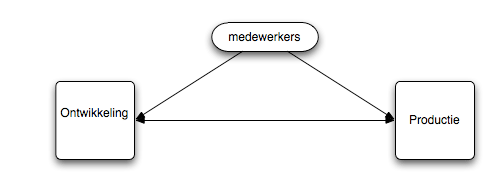
\includegraphics[scale=0.70]{situatie_oud.png}
  \caption[Oude situatie.]{De oude werksituatie bij Fullmoon.}
\end{figure}

\begin{figure}
  \centering
  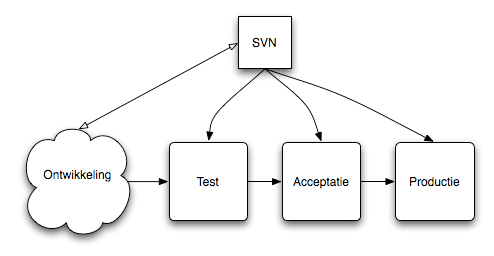
\includegraphics[scale=0.70]{situatie_nieuw.png}
  \caption[Nieuwe situatie.]{De nieuwe situatie.}
\end{figure}

In figuren 2.1 en 2.2 zijn respectievelijk de oude en nieuwe werksituatie bij Fullmoon grafisch uitgewerkt, ik geef hierover een kleine uitleg.

In de oude situatie werkte iedere medewerker via de eigen computer direct op de centrale ontwikkelserver, waarbij men vaak dezelfde bestanden open had staan. Soms werd er ook direct gewerkt op de onlineserver, waardoor er natuurlijk verschillen ontstonden.

In de nieuwe situatie werkt men op zijn eigen computer met gebruikmaking van Subversion (SVN). De ontwikkelomgeving in dit figuur bestaat dus in feite uit de computers van alle medewerkers. Wijzigingen gaan eerst de test- en acceptatieomgevingen door, voordat deze online komen te staan. Er worden dus alleen bestanden aangepast in de ontwikkelomgeving, zodat er nooit verschillende versies onstaan omdat iemand online wat heeft aangepast.
  \chapter{Werkzaamheden}

In dit tweede deel van het projectverslag zal ik kort in kaart brengen wat ik voor mijn afstudeerproject heb gedaan en wat ik hier van opgestoken heb.

\section{Verrichtingen}

Na een half jaar stage had ik al een aardig inzicht gekregen naar de wensen en eisen met betrekking tot de verbetering van de werksituatie. Ik heb getracht om aan de wens van Fullmoon om te komen tot een efficiëntere werkwijze, tegemoet te komen door na te denken over verbeteringen en aanpassingen. Om mijn ideeën hierover te kunnen toetsen heb ik veel kunnen brainstormen met Bart Brugmans, projectmanager bij Fullmoon. Vaak had ik verschillende alternatieven voor een bepaald probleem onderzocht, waarna Bart en ik samen overlegden om tot de beste keuze te komen. Om de voordelen van de door mij voorgestelde aanpassingen duidelijk te maken aan de medewerkers van Fullmoon, heb ik nog tijdens mijn stageperiode een document opgesteld, waarin ik de huidige situatie heb besproken en hoe deze verbeterd kon worden door middel van {\sc scm}. Daarnaast heb ik ook nog een presentatie gegeven over hoe dit in zijn werk zal gaan en heb ik vragen beantwoord. 

Tijdens het project kon ik, nadat in nauw overleg met Fullmoon beslist was over de diverse zaken die moesten worden ingevoerd, zoals het gescheiden werken en gebruik maken van Subversion, overgaan tot het daadwerkelijk inrichten van de situatie.

Zo heb ik een server volledig klaar gemaakt om de Subversion repository en de Redmine site te hosten. Redmine heb ik geconfigureerd naar de wensen van Fullmoon. Zo is er een koppeling met Subversion en maakt het gebruik van de mailfuncties van de server om updates van tickets en dergelijke naar medewerkers te sturen. Op de workstations heb ik overal een webserver geïnstalleerd en heb ik deze klaar gemaakt voor het gebruik van Subversion.

Ook heb ik een tiental lopende projecten in Subversion geïmporteerd en deze zo aangepast dat ze ook van de lokale webserver te draaien zijn. Normaal gezien werkte deze alleen maar vanaf de centrale server. Om de meest gebruikte handelingen zoals het aanmaken van een nieuw project, het importeren van data en het echte werken met Subversion nog meer te verduidelijken heb ik een interne wiki gevuld met informatie. Hier kunnen medewerkers rustig de belangrijkste dingen nalezen mochten ze er niet meer uitkomen.

In overleg met Fullmoon werd beslist dat de situatie klaar was voor gebruik, waarna ik in samenwerking met Bart nog een presentatie heb gegeven. Behalve over Subversion ging deze presentatie over de veranderingen ten opzichte van de oude situatie met betrekking tot de werkwijze en over het gebruik van Redmine.

Naast de uitleg tijdens de presentatie en de informatie op de wikipagina, heb ik ook alle medewerkers een half uur tot een uur individueel begeleid. Hierdoor kregen ze beter in de gaten hoe er in de praktijk met Subversion gewerkt moest worden, want naar een presentatie kijken is toch minder duidelijk dan dat je er zelf mee aan de slag gaat. Ook tijdens deze sessies heb ik nog heel wat vragen beantwoord, waarna ik vragen die vaker gesteld werden nog extra uitgewerkt heb op de wiki. Na een testperiode van enkele weken heb ik de feedback van de medewerkers verzameld om te peilen hoe het een en ander verliep. De meeste reacties waren positief, maar er waren een paar onderdelen waar men nog iets duidelijker uitleg over wilde krijgen, zoals wat te doen bij een conflict in Subversion en hoe men het beste kan branchen. Deze vragen en enkele onderwerpen waarvan ik vermoedde dat men er misschien nog moeite mee had, heb ik verder uitgewerkt en extra belicht op de wikipagina.

\section{Opgestoken kennis}

Afgezien van het feit dat ik nu vrij veel weet op het gebied van het inrichten van een technische infrastructuur, zijn er nog een aantal zaken waar ik tevreden over ben als ik terugkijk naar het project. In principe heb ik het gehele vierde studiejaar goed zelfstandig volbracht. Ik heb een afstudeerproject voorgesteld bij een bedrijf, hun werksituatie in kaart gebracht, adviezen aangedragen om bepaalde zaken te verbeteren en tenslotte een planning opgesteld. Vooral over die planning was ik tevreden, want het bleek een goede te zijn waar ik mij volledig aan heb kunnen houden. In de voorgaande studiejaren was niet altijd de discipline aanwezig om opgestelde planningen te volgen, waardoor het soms nachtwerk werd om een deadline te halen. Ik denk niet dat ik een uitzondering vormde op dit gebied in vergelijking met mijn medestudenten. Natuurlijk heb ik een project uitgevoerd bij een zakelijke instelling, waardoor er wel wat van je verwacht wordt en er een zekere druk op de ketel staat, maar toch ben ik erg tevreden over mijn ontwikkeling op het gebied van discipline en zelfstandigheid.

In het vierde en laatste studiejaar, heb ik het gevoel gekregen dat ik als student meer volwassen ben geworden. Wat dat betreft komt het wel goed overeen met het leerpatroon dat voor de studie is opgesteld.

Naast het vasthouden aan een planning komt deze groei naar volwassenheid mij ook ten goede in andere situaties. Zo heb ik nadat ik de werksituatie bij Fullmoon in kaart had gebracht, mijn visie over de verbetering kunnen geven. In voorgaande jaren had ik er nooit aan gedacht om een bedrijf te kunnen adviseren over hun werksituatie, omdat ik me nog teveel student voelde, terwijl ik me nu een volwaardige collega voel. 

Dit merkte ik ook bij de manier van omgaan met andere medewerkers. Ik heb individueel en in groepen met meer zelfvertrouwen trainingen en uitleg gegeven, zonder aarzeling om mijn mening te laten horen. Tijdens de opleiding wordt wel veel met projecten gewerkt, maar er bestaat toch verschil in het omgaan met studiegenoten en met collega's. Dat ik tijdens mijn stageperiode en afstudeerproject hier veel over heb opgestoken is voor mijn toekomstige carrière erg belangrijk.

  \chapter{Conclusie}

Door een project uit te voeren bij een bedrijf en een adviesrapport op te stellen heb ik mijn afstudeerproject op een iets andere manier aangepakt dan mijn medestudenten. Het ligt niet helemaal in de lijn van een ``echte'' scriptie, maar ik zie dat toch als een voordeel. Het adviesrapport kan ik straks namelijk aan diverse mensen tonen, die daardoor hun eigen situatie kunnen bekijken en vervolgens -- indien nodig -- misschien ook een aantal adviezen kunnen implementeren. Bij een scriptie heb ik toch meer het idee dat het vrij snel op een plank terecht komt, waarna niemand er ooit meer in kijkt.

Naast de mogelijkheid dat er misschien mensen hun voordeel mee kunnen doen, ben ik ook tevreden over het feit dat ik voor Fullmoon echt iets heb kunnen betekenen. Men liep al een tijdje rond met de gedachte om hun manier van werken te verbeteren, maar omdat het zo druk was hadden ze daar geen tijd voor. Bij Fullmoon waren ze dus blij dat iemand van buitenaf hun hierbij kon assisteren. Tijdens mijn afstudeerstage hebben ze mij geweldig geholpen met het delen van hun kennis en ervaring en ik heb het gevoel dat ik dat nu terug heb kunnen betalen.

Ontwikkeling is vaak niet echt tastbaar maar wanneer ik nu terugkijk op het afgelopen jaar, dan wordt het voor mijzelf toch duidelijk dat deze zeker heeft plaatsgevonden. Dankzij de stage en het project heb ik nu het gevoel gekregen dat ik een volwaardige werknemer ben, die een aanwinst kan zijn voor elk bedrijf. Ik voel dat ik er klaar voor ben om te gaan werken en alles in praktijk te brengen wat ik de afgelopen vier jaar via mijn studie aan de Hogeschool van Amsterdam, opleiding Interactieve Media en door de dagelijkse praktijk heb geleerd.


\end{document}
